% Preface required in the knitr RnW file
\documentclass{article}\usepackage[]{graphicx}\usepackage[]{color}
%% maxwidth is the original width if it is less than linewidth
%% otherwise use linewidth (to make sure the graphics do not exceed the margin)
\makeatletter
\def\maxwidth{ %
  \ifdim\Gin@nat@width>\linewidth
    \linewidth
  \else
    \Gin@nat@width
  \fi
}
\makeatother

\definecolor{fgcolor}{rgb}{0.345, 0.345, 0.345}
\newcommand{\hlnum}[1]{\textcolor[rgb]{0.686,0.059,0.569}{#1}}%
\newcommand{\hlstr}[1]{\textcolor[rgb]{0.192,0.494,0.8}{#1}}%
\newcommand{\hlcom}[1]{\textcolor[rgb]{0.678,0.584,0.686}{\textit{#1}}}%
\newcommand{\hlopt}[1]{\textcolor[rgb]{0,0,0}{#1}}%
\newcommand{\hlstd}[1]{\textcolor[rgb]{0.345,0.345,0.345}{#1}}%
\newcommand{\hlkwa}[1]{\textcolor[rgb]{0.161,0.373,0.58}{\textbf{#1}}}%
\newcommand{\hlkwb}[1]{\textcolor[rgb]{0.69,0.353,0.396}{#1}}%
\newcommand{\hlkwc}[1]{\textcolor[rgb]{0.333,0.667,0.333}{#1}}%
\newcommand{\hlkwd}[1]{\textcolor[rgb]{0.737,0.353,0.396}{\textbf{#1}}}%
\let\hlipl\hlkwb

\usepackage{framed}
\makeatletter
\newenvironment{kframe}{%
 \def\at@end@of@kframe{}%
 \ifinner\ifhmode%
  \def\at@end@of@kframe{\end{minipage}}%
  \begin{minipage}{\columnwidth}%
 \fi\fi%
 \def\FrameCommand##1{\hskip\@totalleftmargin \hskip-\fboxsep
 \colorbox{shadecolor}{##1}\hskip-\fboxsep
     % There is no \\@totalrightmargin, so:
     \hskip-\linewidth \hskip-\@totalleftmargin \hskip\columnwidth}%
 \MakeFramed {\advance\hsize-\width
   \@totalleftmargin\z@ \linewidth\hsize
   \@setminipage}}%
 {\par\unskip\endMakeFramed%
 \at@end@of@kframe}
\makeatother

\definecolor{shadecolor}{rgb}{.97, .97, .97}
\definecolor{messagecolor}{rgb}{0, 0, 0}
\definecolor{warningcolor}{rgb}{1, 0, 1}
\definecolor{errorcolor}{rgb}{1, 0, 0}
\newenvironment{knitrout}{}{} % an empty environment to be redefined in TeX

\usepackage{alltt}

\usepackage{rotating}
\usepackage{graphics}
\usepackage{latexsym}
\usepackage{color}
\usepackage{listings} % allows for importing code scripts into the tex file
\usepackage{amsmath}

% Approximately 1 inch borders all around
\setlength\topmargin{-.56in}
\setlength\evensidemargin{0in}
\setlength\oddsidemargin{0in}
\setlength\textwidth{6.49in}
\setlength\textheight{8.6in}

% change name of Abstract
\renewcommand{\abstractname}{Executive Summary}
% allow multiple sections in appendix
\usepackage[title]{appendix}

\title{The Effect of New Housing Projects on Expenditures in Two New York Municipalities} 
\author{Andrew Bates}
\date{October 11, 2018}
\IfFileExists{upquote.sty}{\usepackage{upquote}}{}
\begin{document} 
\maketitle

\begin{abstract}
In this paper we estimate future expenditures for two municipalites in New York based on various projected demographic and income-related factors. These estimates are obtained from a linear regression model chosen via a stepwise model selection procedure. The variables included in the model are wealth per person, population, percent intergovernmental funding, and growth rate. The estimated expenditures for Warwick are \$$261$ per person in $2005$ and \$$271$ per person for $2025$. The estimated expenditures for Monroe are \$$273$ per person for both $2005$ and $2025$. Based on the model, we can infer that increases in population and wealth per person lead to increases in expenditures while increases in intergovernmental funding and growth rate lead to decreases in expenditures.
\end{abstract}


\section{Introduction} \label{intro}

Two New York towns, Warwick and Monroe, would like to estimate future expenditures triggered by new housing construction proposals. They are primarily interested in determining whether they need to increase funds to compensate for increased expenditures related to the housing projects. To construct these estimates, Warwick and Monroe obtained data on expenditures along with various demographic and income-related variables from several New York municiplaties. 


The data used in this study consisted of 916 observations of seven variables. Each observation corresponds to a New York municipality for which each of the variables were collected. The response variable is expenditure per person. The covariates are as follows: wealth per person, population, revenue from state and federal grants, population density, mean income per person, and growth rate.

For reasons of simplicity and interpretability, a linear regression model was chosen to estimate future expenditures. The correlation between population and population density was high ($0.67$) so to prevent this from leading to multicolinearity issues, only population was considered in the analysis. The variables in this data set (including the response) were heavily skewed, so log transformations were applied to each. To ensure a linear relationship between the predictors and the response, the data was subsetted to include only those observations for which the population was larger than $4,000$. The projected covariates for Warwick and Monroe fall within the range of the covariates in the subsetted data so we felt this method was appropriate. In addition, this method was favored over a more complicated method like including a quadratic term on log population which would be harder to interpret. The regression model was constructed via stepwise regression using akaike information criterion (AIC) as the selection criterion. This model was then used to estimate future expenditures.



\section{Analysis} \label{analysis}




\subsection{Exploratory Analysis} \label{eda}

In this data set there were two measures of the size of a municipality: population and population density. Unsurprisingly, the correlation between these two measures was relatively high ($0.67$). In the interest of parsimony and to mitigate possible colinearity issues, we decided to consider only one of these variables to construct our model. Population density had a moderate correlation with mean income per person ($0.49$) whereas population had a comparably low correlation with income ($0.29$). To hedge against problems with colinearity, we decided to consider population for the model building process.

Upon an initial examination of the data, it was evident that transformations would be necessary. Each of the covariates, and the response, were skewed (see Appendix \ref{appendix_plots}) and some were heavily skewed. As this might pose problems with linearity, we performed transformations on the variables. To remain in line with our goal of having a comprehensible model, we favored log transformations over a more complex procedure. To that end, we performed log transformations on all variables in the data set.  However, a straightforward application of the logarithm was not possible for one covariate. Growth rate contains some negative values as well as some zero values. To remedy this, we used the following pseudo-log transformation:
\[
\text{p-}\log(\text{growth rate}) = % plog for pseudo-log
  \begin{cases}
    \log(\text{growth rate} + 0.15) &\text{if growth rate} > 0 \\
    -\log(-\text{growth rate} + 0.15) &\text{if growth rate} \le 0.
  \end{cases}
\]
Note that since this is a one-to-one transformation ...

To ensure the linearity assumption of our model was satisfied, we examined the relationship between log expenditure and the log of each of the covariates. Except for log population, all other covariates had an approximately liner relationship with log expenditure. Figure \ref{fig:vs_log_pop} is a plot of log expenditure vs. log population with the addition of a smoothing line. We see what appears to be a quadratic relationship. However, notice that on either side of the vertical line (corresponding to a log population of $8.3$), the relationship is approximately linear. So we were essentially faced with two choices. We could try to include the square of log population as an additional predictor or we could subset the data and have a roughly linear relationship between the response and log population.


\begin{knitrout}
\definecolor{shadecolor}{rgb}{0.969, 0.969, 0.969}\color{fgcolor}\begin{figure}[h]
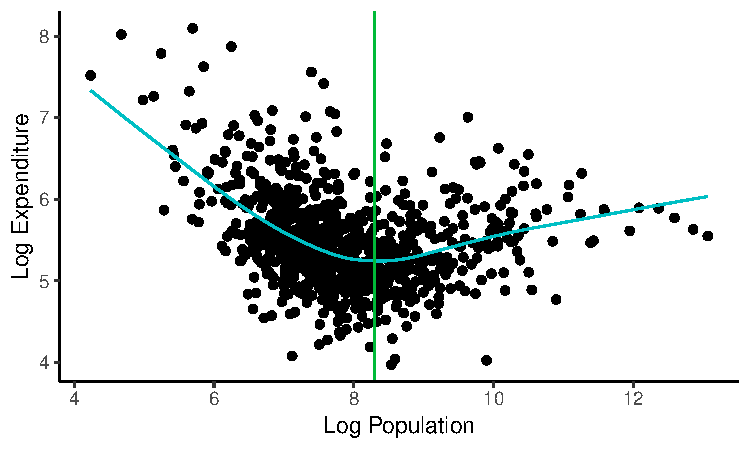
\includegraphics[width=\maxwidth]{figure/r_fig_vs_log_pop-1} \caption{\label{fig:vs_log_pop} Plot of log expenditure vs. log population with LOWESS smooth line}\label{fig:r fig_vs_log_pop}
\end{figure}


\end{knitrout}

We chose the latter method. As mentioned previously, we favored a simpler model for the interpretability that comes with it. The log of population squared is not as easy to understand. Also, the projected covariates we would be predicting with fall within the rang of the covariates in the subsetted data. For these reasons, we subsetted the data to include only those observations that had a population greater than $4,000$ (log population above $8.3$). This subsetted data set included $266$ of the original observations which we felt was large enough to obtain reliable inferences from. Figure \ref{fig:vs_log_pop_subset} is a plot of log expenditure vs. log population for this subsetted data set along with a smoothing line. We can see that the relationship between the two variables is roughly linear. We do see minor deviation from linearity for high values of log population but overall the trend is approximately linear. Additionally, it is much more linear than the relationship we see in Figure \ref{fig:vs_log_pop}.

\begin{knitrout}
\definecolor{shadecolor}{rgb}{0.969, 0.969, 0.969}\color{fgcolor}\begin{figure}[h]
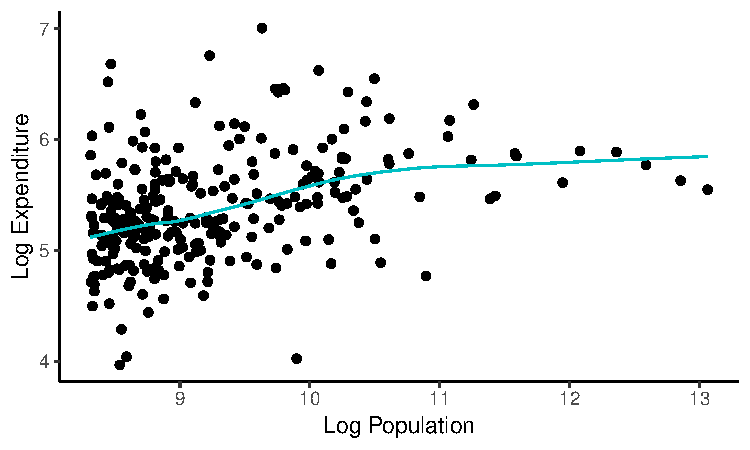
\includegraphics[width=\maxwidth]{figure/r_fig_vs_log_pop_subset-1} \caption{\label{fig:vs_log_pop_subset} Plot of log expenditure vs. log population with LOWESS smooth line from subsetted data}\label{fig:r fig_vs_log_pop_subset}
\end{figure}


\end{knitrout}

\subsection{Modeling and Diagnostics} \label{modeling}

After performing variable transformations and data subsetting, our regression model was ready to be constructed. We used both forward and backward stepwise regression to build the model. AIC was used as our model selection criterion. This was partly due to the ubiquity of AIC and partly because it penalizes larger models. This penalization aligns itself with our preference for simpler models. That being said, we did investigate the inclusion of squared log transformations for all the covariates ($\log^2(\text{income})$, etc.). However, there was not much of an improvement that could be gained by including these terms. The AIC for the model including these terms was $-622$ while the AIC for the model without them was $-611$, not much of a difference. Furthermore, the model with the quadratic variables included contained some quadratic terms without their corresponding linear components. We simply could not justify such a model. The final model used log expenditure as the response with the following covariates: log wealth, log population, log percent intergovernmental funding, and log growth rate.

Diagnostic plots from the fitted model are shown in Figure \ref{fig:diag}. The left figure is a plot of studentized residuals vs. fitted values. The horizontal line is a reference line at a residual of zero. Notice that there are no apparent patterns and the points are scattered roughly equally about the reference line. Nevertheless, there is a troublesome point with an unusually small value. This point corresponds to a municipality with a rather large value of wealth per person. It's not entirely surprising that such a municipality exists as wealth related data often contains abnormally high observations. Although this observation is a bit outside the range of most of the data, it is nonetheless a valid data point and this municipality may also wish to estimate their future expenditures at some point. For this reason, we decided to not remove this data point. The right-hand side of figure \ref{fig:diag} provides an alternative view of the model residuals. Here we have plotted quantiles of the studentized residuals against quantiles of a $t$ distribution which is the distribution that they should follow theoretically. The blue line is a reference line, indicating what the theoretical relationship should be. Aside from the point just discussed, we see that the residuals follow their theoretical distribution quite well. As an additional diagnostic assessment, we computed variance inflation factors which were all less than $1.2$. Considering our diagnostic plots and metrics as a whole, we were satisfied with this model.


\begin{knitrout}
\definecolor{shadecolor}{rgb}{0.969, 0.969, 0.969}\color{fgcolor}\begin{figure}
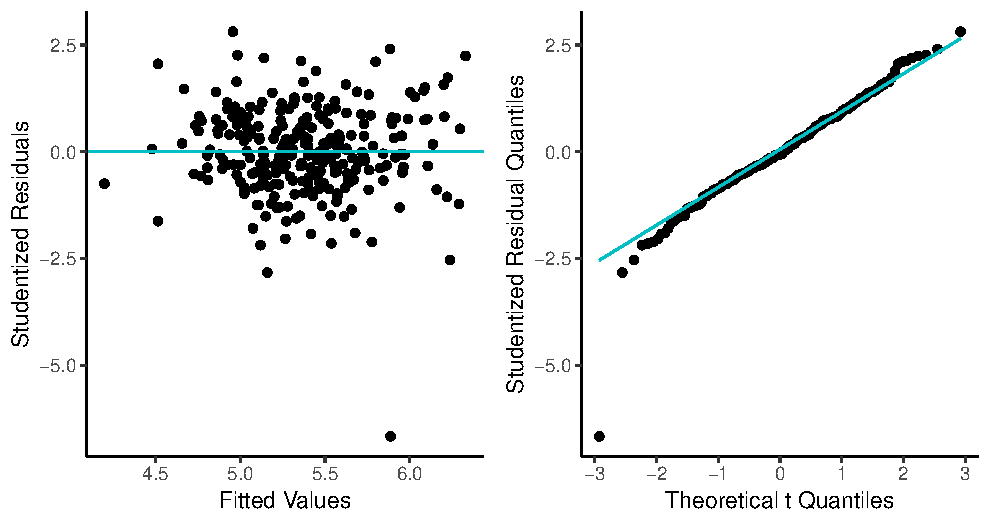
\includegraphics[width=\maxwidth]{figure/r_diag_plots-1} \caption{\label{fig:diag} Diagnostic plots for regression model. The left plot shows studentized residuals vs. fitted values. The right plot shows a QQ plot of the studentized residuals vs. t-distribution quantiles.}\label{fig:r diag_plots}
\end{figure}


\end{knitrout}

A summary of the regression model can be found in Table \ref{tbl:regress}. Note that all p-values (except the intercept) significant at the $0.05$ level and the $95$\% confidence intervals are relatively narrow. The largest coefficient is for wealth per person which is $0.49$ on the log scale. We can interpret this as follows. For a \$$1,000$ increase in the wealth per person, the municipality can expect expenditures to increase by \$$30$ per person, provided the other covariates remain constant. This may seem odd in that one might expect wealtier people to require less money from their local government. But perhaps the increase in expenditures comes from providing additional community resources, infrastracture improvements, or increased funding for public schools. Increased expenditures on items such as these tend to be more common in wealthier areas compared to their less wealthy counterparts. The values of the remaining coefficients can be interpreted in a similar manner. But note that the signs of the coefficients for the other covariates are a bit more inline with what we might initially expect. A municipality with a larger population will likely need to spend more money than a smaller one. The more funding a local municipality receives from state and federal governments, the less they will need to spend themselves. A town that sees a quick influx of new residents will probably require increased expenditures eventually but given the typical pace of government entities, this increase will not be immediate.

% one unit increase in wealth corresponds to $1,000 increase
% one unit increase in wealth = log(1000) = 0.69 unit increase in log expend
%  = 6.9 * 0.49 = 3.4 increase in log expend
%  = exp(3.4) = 30 unit increase in expenditure
%  = $30 increase in expenditure per person



% latex table generated in R 3.5.1 by xtable 1.8-3 package
% Tue Oct  9 19:12:31 2018
\begin{table}[ht]
\centering
\begin{tabular}{|l|rrrr|}
  \hline
 & Estimate & SE & p-value & 95\% CI \\ 
  \hline
Intercept & 0.13 & 0.44 & 0.769 & ( -0.731 , 0.987 ) \\ 
  Log Wealth & 0.49 & 0.04 & 0.000 & ( 0.423 , 0.563 ) \\ 
  Log Population & 0.08 & 0.02 & 0.001 & ( 0.032 , 0.123 ) \\ 
  Log \% Intergov Funding & -0.28 & 0.04 & 0.000 & ( -0.358 , -0.198 ) \\ 
  Log Growth Rate & -0.02 & 0.01 & 0.031 & ( -0.046 , -0.002 ) \\ 
   \hline
\end{tabular}
\caption{Summary table for regressing log expenditure on log wealth, log population, log percent intergovernmental funding, and log growth rate.} 
\label{tbl:regress}
\end{table}



\subsection{Predictions}

The projections for Warwick and Monroe in $2005$ and $2025$, along with expenditure predictions and prediction intervals, can be found in Table \ref{tbl:pred}. The most obvious thing to note is the the estimated expenditure for Monroe is the same in $2005$ and $2025$. The increased expenditures from rising population and wealth from $2005$ to $2025$ is probably offset by the decrease in expenditure from rising intergovermental funding rate. The net effect being that the predicted expentures remain the same. Warwick on the other hand, is projected to see larger increases in population and wealth over the twenty year period than Monroe will. These large increases are not offset by the decrease in expenditure due to rising intergovernmental funding and growth rate which leads to an increase in expenditures over the same period of \$$10$ per person. Although Warwick should expect to see their expenditures rise, by $2025$ we expect to see roughly the same expenditure per person for both towns.

% latex table generated in R 3.5.1 by xtable 1.8-3 package
% Wed Oct 10 16:01:26 2018
\begin{table}[ht]
\centering
\begin{tabular}{|l|rrrrrr|}
  \hline
 & Population & Wealth & \% Intergov Funding & Growth Rate & Estimate & 95 \% PI \\ 
  \hline
Warwick-2005 & 20442 & 85000 & 25.0 & 35.0 & 261 & ( 139 , 489 ) \\ 
  Warwick-2025  & 31033 & 89000 & 26.0 & 40.0 & 271 & ( 144 , 509 ) \\ 
  Monroe-2005 & 10496 & 58000 & 8.8 & 35.0 & 273 & ( 147 , 510 ) \\ 
  Monroe-2025 & 13913 & 60000 & 10.0 & 35.0 & 273 & ( 147 , 510 ) \\ 
   \hline
\end{tabular}
\caption{Projections for Warwick and Monroe along with predicted expenditures and prediction intervals.} 
\label{tbl:pred}
\end{table}




\section{Conclusion} \label{conclusion}

In this paper we developed a linear regression model in order to estimate future expenditures for two New York municipalities, Warwick and Monroe. The model was constructed via a stepwise regression procedure with the final model containg the following covariates: population, wealth per person, percent intergovernment funding, and growth rate. The model suggests that a rise in either population or growth rate will contribute to a rise in expenditures. On the other hand, a rise in intergovernmental funding or growth rate will lead to a decrease in expenditures. The predicted expenditures for Warwick are \$$261$ per person in $2005$ and \$$271$ per person for $2025$. The estimated expenditures for Monroe are \$$273$ per person for both $2005$ and $2025$.



\newpage
\begin{appendices}

\section{Supplementary Plots} \label{appendix_plots}


\begin{knitrout}
\definecolor{shadecolor}{rgb}{0.969, 0.969, 0.969}\color{fgcolor}\begin{figure}[h!]
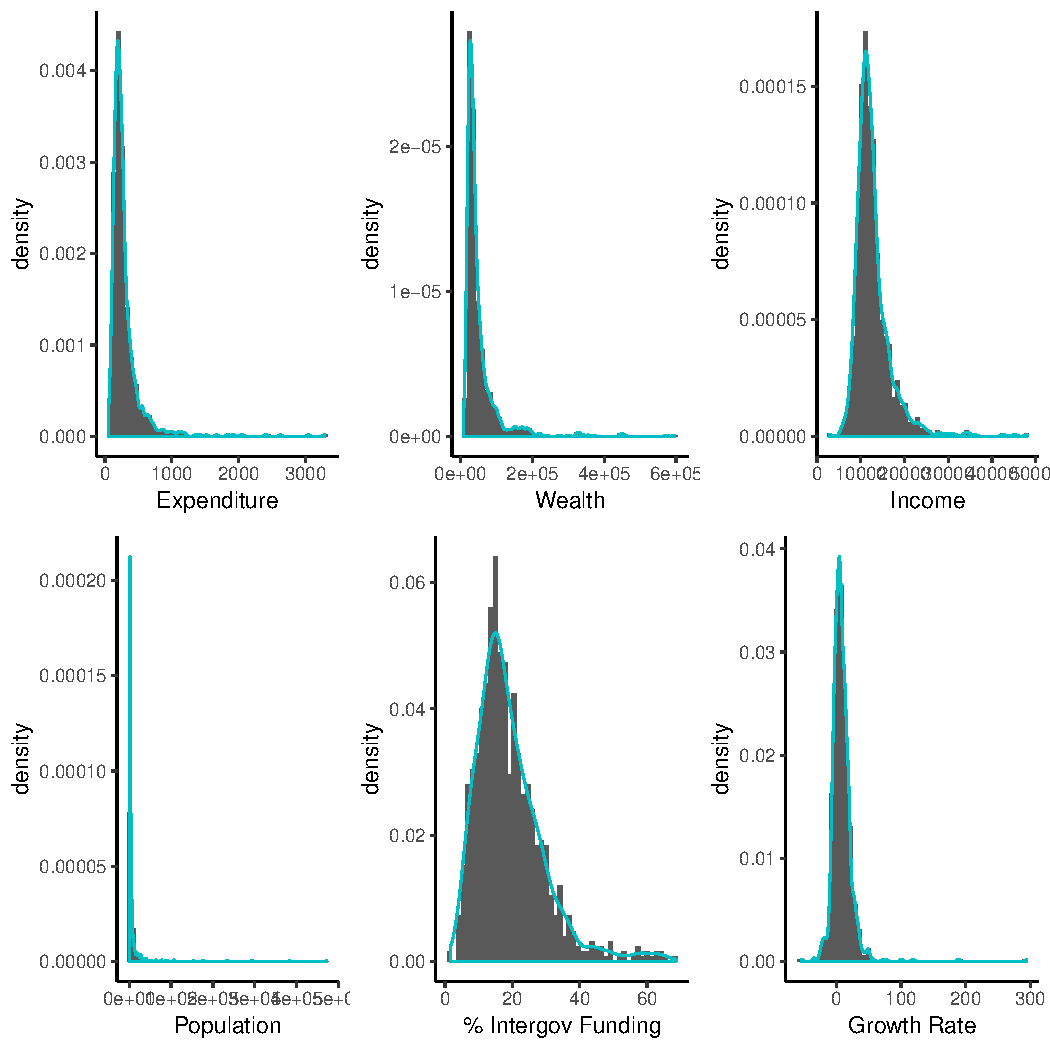
\includegraphics[width=\maxwidth]{figure/r_append_hist-1} \caption[Histograms of all variables with densities overlayed]{Histograms of all variables with densities overlayed.}\label{fig:r append_hist}
\end{figure}


\end{knitrout}



\begin{knitrout}
\definecolor{shadecolor}{rgb}{0.969, 0.969, 0.969}\color{fgcolor}\begin{figure}
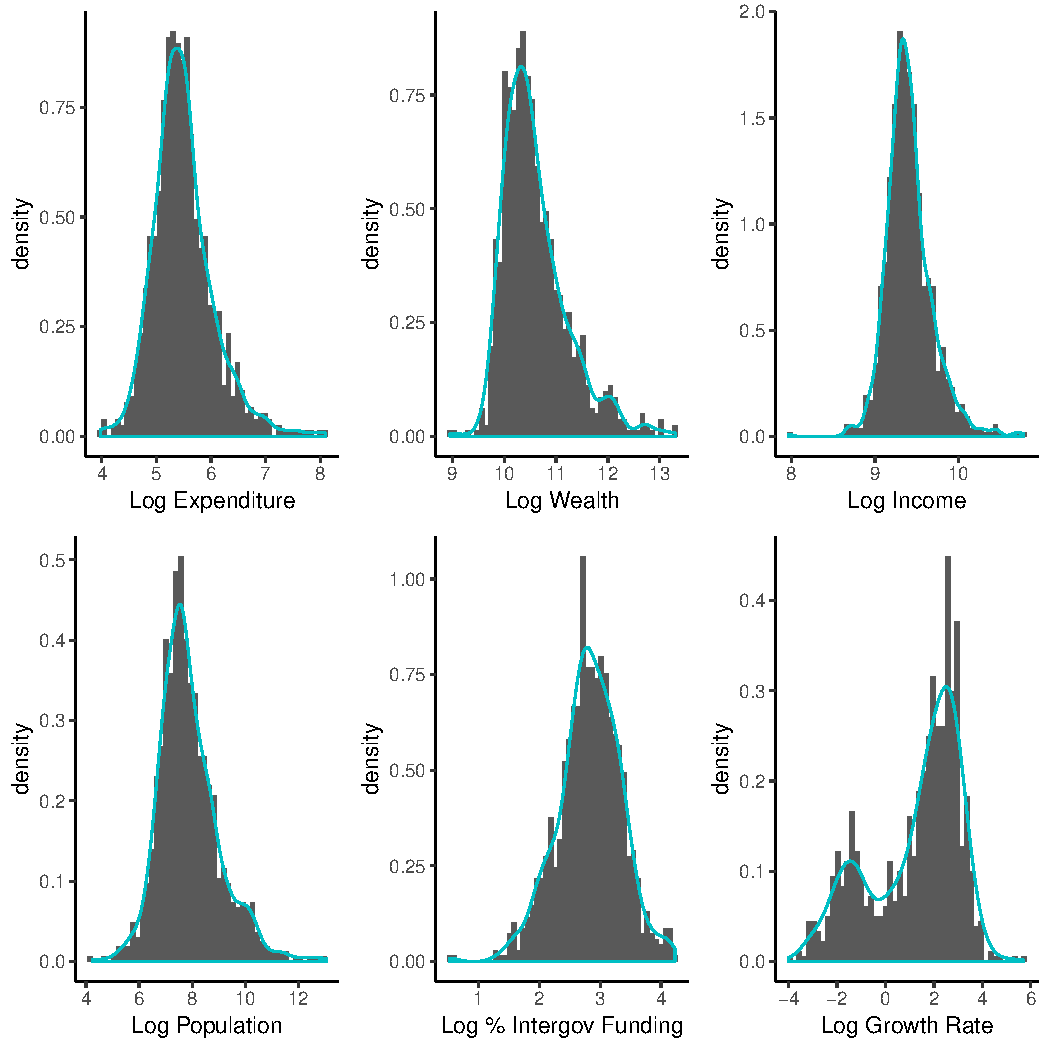
\includegraphics[width=\maxwidth]{figure/r_append_log_hist-1} \caption[Histograms of log transformed variables with densities overlayed]{Histograms of log transformed variables with densities overlayed.}\label{fig:r append_log_hist}
\end{figure}


\end{knitrout}


\begin{knitrout}
\definecolor{shadecolor}{rgb}{0.969, 0.969, 0.969}\color{fgcolor}\begin{figure}
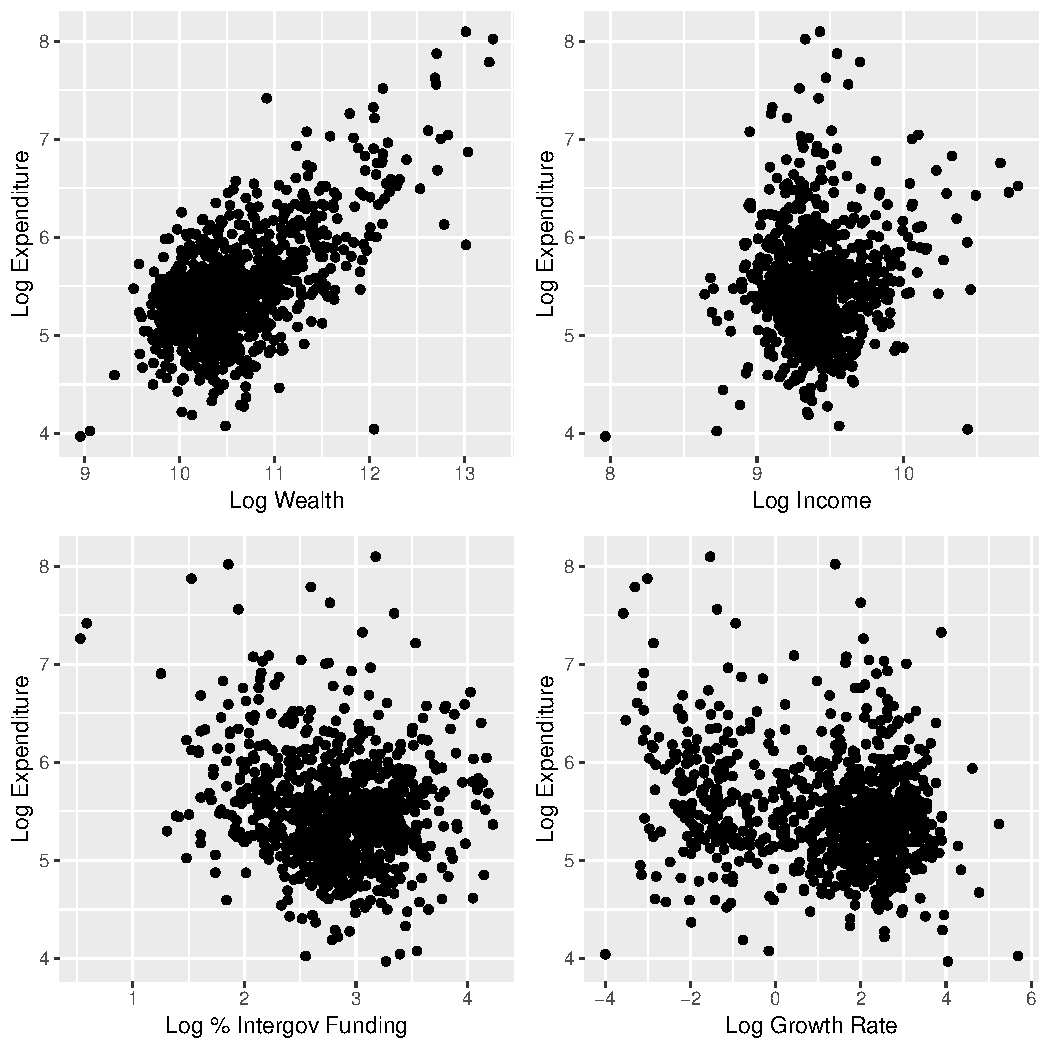
\includegraphics[width=\maxwidth]{figure/r_append_scatter-1} \caption[Scatter plots of log expenditure vs]{Scatter plots of log expenditure vs. log covariate for each covariate except population (see main text).}\label{fig:r append_scatter}
\end{figure}


\end{knitrout}


\newpage
\section{R Code}
\begin{knitrout}
\definecolor{shadecolor}{rgb}{0.969, 0.969, 0.969}\color{fgcolor}\begin{kframe}
\begin{alltt}
\hlkwd{library}\hlstd{(readr)} \hlcom{# read in data}
\hlkwd{library}\hlstd{(dplyr)} \hlcom{# data manipulation}
\hlkwd{library}\hlstd{(corrplot)} \hlcom{# correlation plotting}
\hlkwd{library}\hlstd{(ggplot2)} \hlcom{# plotting}
\hlkwd{library}\hlstd{(MASS)} \hlcom{# stepwise regression}
\hlkwd{library}\hlstd{(car)} \hlcom{# regression helper}
\hlkwd{library}\hlstd{(broom)} \hlcom{# tidy model output}
\hlkwd{library}\hlstd{(here)} \hlcom{# file path helper}
\hlkwd{library}\hlstd{(xtable)} \hlcom{# table formatting}

\hlstd{ny} \hlkwb{<-} \hlkwd{read_csv}\hlstd{(}\hlkwd{here}\hlstd{(}\hlstr{"reports/ny_expenditure/ny_expend.csv"}\hlstd{))}

\hlcom{# =======================================================}
\hlcom{# ----------------- EDA ------------------------}
\hlcom{# =======================================================}

\hlcom{# ------ numerical summaries --------}
\hlstd{ny} \hlkwb{<-} \hlkwd{filter}\hlstd{(ny,} \hlopt{!}\hlkwd{is.na}\hlstd{(expenditure))} \hlcom{# remove 2 rows with missing values}
\hlkwd{dim}\hlstd{(ny)} \hlcom{# 914 x 7}
\hlkwd{summary}\hlstd{(ny)}
\hlstd{corr_mat} \hlkwb{<-} \hlkwd{cor}\hlstd{(ny)}
\hlkwd{corrplot}\hlstd{(corr_mat,} \hlkwc{type} \hlstd{=} \hlstr{"upper"}\hlstd{,} \hlkwc{diag} \hlstd{=} \hlnum{FALSE}\hlstd{)} \hlcom{# correlation matrix plot}

\hlcom{# highest correlations}
\hlkwd{cor}\hlstd{(ny}\hlopt{$}\hlstd{pop, ny}\hlopt{$}\hlstd{pop_dens)} \hlcom{# 0.67}
\hlkwd{cor}\hlstd{(ny}\hlopt{$}\hlstd{income, ny}\hlopt{$}\hlstd{pop_dens)} \hlcom{# 0.49}
\hlkwd{cor}\hlstd{(ny}\hlopt{$}\hlstd{income, ny}\hlopt{$}\hlstd{perc_intergov)} \hlcom{# -0.30}
\hlkwd{cor}\hlstd{(ny}\hlopt{$}\hlstd{income, ny}\hlopt{$}\hlstd{pop)} \hlcom{# 0.29}

\hlstd{ny} \hlkwb{<-} \hlstd{ny} \hlopt
  \hlstd{dplyr}\hlopt{::}\hlkwd{select}\hlstd{(}\hlopt{-}\hlstd{pop_dens)} \hlcom{# remove population density}

\hlcom{# ---  histograms and density plots ----}

\hlcom{# function to create histogram and density given variable name}
\hlcom{# as is, it's really only useful in this script}
\hlstd{hist_dens} \hlkwb{<-} \hlkwa{function}\hlstd{(}\hlkwc{var}\hlstd{)\{}
  \hlstd{plot_var} \hlkwb{<-} \hlkwd{enquo}\hlstd{(var)}
  \hlkwd{ggplot}\hlstd{(ny,} \hlkwd{aes}\hlstd{(}\hlkwc{x} \hlstd{=} \hlopt{!!} \hlstd{plot_var,} \hlkwc{y} \hlstd{= ..density..))} \hlopt{+}
    \hlkwd{geom_histogram}\hlstd{(}\hlkwc{bins} \hlstd{=} \hlnum{50}\hlstd{)} \hlopt{+}
    \hlkwd{geom_density}\hlstd{()}
\hlstd{\}}

\hlkwd{hist_dens}\hlstd{(expenditure)}
\hlkwd{hist_dens}\hlstd{(wealth)}
\hlkwd{hist_dens}\hlstd{(income)}
\hlkwd{hist_dens}\hlstd{(pop)}
\hlkwd{hist_dens}\hlstd{(perc_intergov)}
\hlkwd{hist_dens}\hlstd{(grow_rate)}

\hlcom{# all variables are right-skewed so we log transform them all}
\hlcom{# however, since growth rate contains negative values,}
\hlcom{# we use a modified log transform}
\hlstd{ny} \hlkwb{<-} \hlstd{ny} \hlopt
  \hlkwd{mutate}\hlstd{(}
    \hlkwc{log_expenditure} \hlstd{=} \hlkwd{log}\hlstd{(expenditure),}
    \hlkwc{log_wealth} \hlstd{=} \hlkwd{log}\hlstd{(wealth),}
    \hlkwc{log_income} \hlstd{=} \hlkwd{log}\hlstd{(income),}
    \hlkwc{log_pop} \hlstd{=} \hlkwd{log}\hlstd{(pop),}
    \hlkwc{log_perc_intergov} \hlstd{=} \hlkwd{log}\hlstd{(perc_intergov),}
    \hlkwc{log_grow_rate} \hlstd{=} \hlkwd{ifelse}\hlstd{(grow_rate} \hlopt{>} \hlnum{0}\hlstd{,}
                           \hlkwd{log}\hlstd{(grow_rate} \hlopt{+} \hlnum{0.15}\hlstd{),}
                           \hlopt{-}\hlkwd{log}\hlstd{(}\hlopt{-}\hlstd{grow_rate} \hlopt{+} \hlnum{0.15}\hlstd{))}
  \hlstd{)}

\hlkwd{hist_dens}\hlstd{(log_expenditure)}
\hlkwd{hist_dens}\hlstd{(log_wealth)}
\hlkwd{hist_dens}\hlstd{(log_income)}
\hlkwd{hist_dens}\hlstd{(log_pop)}
\hlkwd{hist_dens}\hlstd{(log_perc_intergov)}
\hlkwd{hist_dens}\hlstd{(log_grow_rate)}


\hlcom{# ---  scatterplots: response vs. predictors ----}

\hlcom{# function to create scatterplot of log expenditure vs. log covariate given}
\hlcom{# covariate name. also adds a scatter plot smooth}
\hlstd{scatter_smooth_log} \hlkwb{<-} \hlkwa{function}\hlstd{(}\hlkwc{var}\hlstd{)\{}
  \hlstd{x_var} \hlkwb{<-} \hlkwd{enquo}\hlstd{(var)}
  \hlkwd{ggplot}\hlstd{(ny,} \hlkwd{aes}\hlstd{(}\hlkwc{x} \hlstd{=} \hlopt{!!} \hlstd{x_var,} \hlkwc{y} \hlstd{= log_expenditure))} \hlopt{+}
    \hlkwd{geom_point}\hlstd{()}
\hlstd{\}}

\hlkwd{scatter_smooth_log}\hlstd{(log_wealth)}
\hlkwd{scatter_smooth_log}\hlstd{(log_income)}
\hlkwd{scatter_smooth_log}\hlstd{(log_pop)}
\hlkwd{scatter_smooth_log}\hlstd{(log_perc_intergov)}
\hlkwd{scatter_smooth_log}\hlstd{(log_grow_rate)}

\hlcom{# all the above plots show an approximatley linear relationship }
\hlcom{# except log expenditure vs. log population}
\hlcom{# in the following plot, it looks like if we might be able to}
\hlcom{# split log population into 2 groups and get an approximately linear relation}

\hlstd{lpop_smooth} \hlkwb{<-} \hlkwd{lowess}\hlstd{(ny}\hlopt{$}\hlstd{log_pop, ny}\hlopt{$}\hlstd{log_expenditure)}

\hlkwd{ggplot}\hlstd{(ny,} \hlkwd{aes}\hlstd{(}\hlkwc{x} \hlstd{= log_pop,} \hlkwc{y} \hlstd{= log_expenditure))} \hlopt{+}
  \hlkwd{geom_point}\hlstd{()} \hlopt{+}
  \hlkwd{geom_line}\hlstd{(}\hlkwd{aes}\hlstd{(}\hlkwc{x} \hlstd{= lpop_smooth}\hlopt{$}\hlstd{x,} \hlkwc{y} \hlstd{= lpop_smooth}\hlopt{$}\hlstd{y),} \hlkwc{color} \hlstd{=} \hlstr{"#00BFC4"}\hlstd{)} \hlopt{+}
  \hlkwd{geom_segment}\hlstd{(}\hlkwd{aes}\hlstd{(}\hlkwc{x} \hlstd{=} \hlnum{8.3}\hlstd{,} \hlkwc{xend} \hlstd{=} \hlnum{8.3}\hlstd{,} \hlkwc{y} \hlstd{=} \hlnum{4}\hlstd{,} \hlkwc{yend} \hlstd{=} \hlnum{5.24}\hlstd{),} \hlkwc{color} \hlstd{=} \hlstr{"#00BA38"}\hlstd{)}

\hlstd{ny_low} \hlkwb{<-} \hlstd{ny} \hlopt
  \hlkwd{filter}\hlstd{(log_pop} \hlopt{<=} \hlnum{8.3}\hlstd{)}

\hlstd{ny_high} \hlkwb{<-} \hlstd{ny} \hlopt
  \hlkwd{filter}\hlstd{(log_pop} \hlopt{>} \hlnum{8.3}\hlstd{)}
\hlkwd{dim}\hlstd{(ny_high)} \hlcom{# 266  12}

\hlkwd{ggplot}\hlstd{(ny_low,} \hlkwd{aes}\hlstd{(}\hlkwc{x} \hlstd{= log_pop,} \hlkwc{y} \hlstd{= log_expenditure))} \hlopt{+}
  \hlkwd{geom_point}\hlstd{()} \hlopt{+}
  \hlkwd{geom_smooth}\hlstd{(}\hlkwc{method} \hlstd{= loess,} \hlkwc{formula} \hlstd{= y} \hlopt{~} \hlstd{x)}

\hlstd{lpop_high_smooth} \hlkwb{<-} \hlkwd{lowess}\hlstd{(ny_high}\hlopt{$}\hlstd{log_pop, ny_high}\hlopt{$}\hlstd{log_expenditure)}

\hlkwd{ggplot}\hlstd{(ny_high,} \hlkwd{aes}\hlstd{(}\hlkwc{x} \hlstd{= log_pop,} \hlkwc{y} \hlstd{= log_expenditure))} \hlopt{+}
  \hlkwd{geom_point}\hlstd{()} \hlopt{+}
  \hlkwd{geom_line}\hlstd{(}\hlkwd{aes}\hlstd{(}\hlkwc{x} \hlstd{= lpop_high_smooth}\hlopt{$}\hlstd{x,}
                \hlkwc{y} \hlstd{= lpop_high_smooth}\hlopt{$}\hlstd{y),} \hlkwc{color} \hlstd{=} \hlstr{"#00BFC4"}\hlstd{)}

\hlcom{# based on the above plots, it appears that the relationship between}
\hlcom{# log expenditure and log population is approximately piecewise linear}

\hlcom{# =======================================================}
\hlcom{# ----------------- model building ----------------------}
\hlcom{# =======================================================}

\hlcom{# we will use stepwise regression for model selection}
\hlcom{# with AIC as our criteria}
\hlcom{# we consider quadratic log terms in the model }
\hlcom{# mostly just to see what the results are}
\hlstd{for_mod_fit_high} \hlkwb{<-} \hlstd{ny_high} \hlopt
  \hlstd{dplyr}\hlopt{::}\hlkwd{select}\hlstd{(log_expenditure,}
                \hlstd{log_wealth,}
                \hlstd{log_income,}
                \hlstd{log_pop,}
                \hlstd{log_perc_intergov,}
                \hlstd{log_grow_rate)} \hlopt
  \hlkwd{mutate}\hlstd{(}
    \hlkwc{log_wealth_2} \hlstd{= log_wealth}\hlopt{^}\hlnum{2}\hlstd{,}
    \hlkwc{log_income_2} \hlstd{= log_income}\hlopt{^}\hlnum{2}\hlstd{,}
    \hlkwc{log_pop_2} \hlstd{= log_pop}\hlopt{^}\hlnum{2}\hlstd{,}
    \hlkwc{log_perc_intergov_2} \hlstd{= log_perc_intergov}\hlopt{^}\hlnum{2}\hlstd{,}
    \hlkwc{log_grow_rate_2} \hlstd{= log_grow_rate}\hlopt{^}\hlnum{2}
  \hlstd{)}

\hlcom{# fit model without quadratic terms}
\hlcom{# best AIC is -611.3}
\hlstd{fit_high} \hlkwb{<-} \hlkwd{lm}\hlstd{(log_expenditure} \hlopt{~} \hlstd{log_wealth} \hlopt{+}
                 \hlstd{log_income} \hlopt{+}
                 \hlstd{log_pop} \hlopt{+}
                 \hlstd{log_perc_intergov} \hlopt{+}
                 \hlstd{log_grow_rate,}
               \hlkwc{data} \hlstd{= for_mod_fit_high)}
\hlstd{best_fit_high} \hlkwb{<-} \hlkwd{stepAIC}\hlstd{(fit_high)}
\hlstd{best_fit_high}

\hlcom{# fit model with quadratic terms}
\hlcom{# best AIC is -622.91}
\hlcom{# this model is not used because:}
\hlcom{# there isn't much of an improvement in AIC compared to the simpler model above}
\hlcom{# this model includes quadratic terms without their respective linear terms}
\hlcom{# we just can not justify such a model}
\hlstd{full_fit} \hlkwb{<-} \hlkwd{lm}\hlstd{(log_expenditure} \hlopt{~}\hlstd{.,} \hlkwc{data} \hlstd{= for_mod_fit_high)}
\hlstd{best_full_fit} \hlkwb{<-} \hlkwd{stepAIC}\hlstd{(full_fit)}
\hlstd{best_full_fit}

\hlstd{final_fit} \hlkwb{<-} \hlkwd{lm}\hlstd{(log_expenditure} \hlopt{~}
                  \hlstd{log_wealth} \hlopt{+}
                  \hlstd{log_pop} \hlopt{+}
                  \hlstd{log_perc_intergov} \hlopt{+}
                  \hlstd{log_grow_rate,}
                \hlkwc{data} \hlstd{= ny_high)}

\hlcom{# =======================================================}
\hlcom{# ----------------- model diagnostics -------------------}
\hlcom{# =======================================================}


\hlcom{# --------------- diagnostic plots ----------------}

\hlcom{# add fitted values, residuals, etc. to orignal data frame used to fit the model}
\hlstd{ny_high} \hlkwb{<-} \hlkwd{augment}\hlstd{(final_fit)} \hlcom{# (broom package)}

\hlcom{# add studentized residuals to data frame}
\hlstd{ny_high} \hlkwb{<-} \hlstd{ny_high} \hlopt
  \hlkwd{mutate}\hlstd{(}\hlkwc{stud_res} \hlstd{=} \hlkwd{rstudent}\hlstd{(final_fit))}

\hlcom{# studentized residuals vs. fitted}
\hlkwd{ggplot}\hlstd{(ny_high,} \hlkwd{aes}\hlstd{(}\hlkwc{x} \hlstd{= .fitted,} \hlkwc{y} \hlstd{= stud_res))} \hlopt{+}
  \hlkwd{geom_point}\hlstd{()} \hlopt{+}
  \hlkwd{geom_hline}\hlstd{(}\hlkwc{yintercept} \hlstd{=} \hlnum{0}\hlstd{)}

\hlcom{# qq plot studentized residuals vs. t distribution}
\hlstd{dist_pars} \hlkwb{=} \hlkwd{list}\hlstd{(}\hlkwc{df} \hlstd{= final_fit}\hlopt{$}\hlstd{df.residual)}
\hlstd{ny_high} \hlopt
  \hlkwd{mutate}\hlstd{(}\hlkwc{stud} \hlstd{=} \hlkwd{rstudent}\hlstd{(final_fit))} \hlopt
  \hlkwd{ggplot}\hlstd{(}\hlkwd{aes}\hlstd{(}\hlkwc{sample} \hlstd{= stud))} \hlopt{+}
  \hlkwd{stat_qq}\hlstd{(}\hlkwc{distribution} \hlstd{= qt,} \hlkwc{dparams} \hlstd{= dist_pars[[}\hlstr{"df"}\hlstd{]])} \hlopt{+}
  \hlkwd{stat_qq_line}\hlstd{(}\hlkwc{distribution} \hlstd{= qt,} \hlkwc{dparams} \hlstd{= dist_pars[[}\hlstr{"df"}\hlstd{]])}

\hlcom{# row with smallest studentized residual}
\hlstd{ny_high} \hlopt
  \hlkwd{filter}\hlstd{(stud_res} \hlopt{==} \hlkwd{min}\hlstd{(stud_res))}

\hlstd{ny_high} \hlopt
  \hlkwd{filter}\hlstd{(stud_res} \hlopt{==} \hlkwd{min}\hlstd{(stud_res))} \hlopt
  \hlstd{dplyr}\hlopt{::}\hlkwd{select}\hlstd{(stud_res)}

\hlcom{# ----- regression summaries -------}

\hlcom{# all p-values (except intercept) are significant at the 0.05 level}
\hlcom{# F test significant at 0.05 level}
\hlkwd{summary}\hlstd{(final_fit)}

\hlcom{# all VIF's are less than 1.2}
\hlkwd{vif}\hlstd{(final_fit)}  \hlcom{# (car package)}


\hlcom{# the following code is mostly just formatting}
\hlstd{ci_bounds} \hlkwb{=} \hlkwd{formatC}\hlstd{(}\hlkwd{signif}\hlstd{(}\hlkwd{confint}\hlstd{(final_fit),} \hlkwc{digits} \hlstd{=} \hlnum{6}\hlstd{),}
                   \hlkwc{digits} \hlstd{=} \hlnum{2}\hlstd{,} \hlkwc{format} \hlstd{=} \hlstr{"f"}\hlstd{,} \hlkwc{flag} \hlstd{=} \hlstr{"#"}\hlstd{)}

\hlstd{regress_tbl} \hlkwb{<-} \hlkwd{tidy}\hlstd{(final_fit)} \hlopt \hlcom{# from broom}
  \hlstd{dplyr}\hlopt{::}\hlkwd{select}\hlstd{(}\hlopt{-}\hlstd{statistic)} \hlopt
  \hlkwd{bind_cols}\hlstd{(}\hlkwc{`95% CI`} \hlstd{=} \hlkwd{paste}\hlstd{(}\hlstr{"("}\hlstd{, ci_bounds[,}\hlnum{1}\hlstd{],} \hlstr{","}\hlstd{, ci_bounds[,}\hlnum{2}\hlstd{],} \hlstr{")"}\hlstd{))} \hlopt
  \hlkwd{mutate}\hlstd{(}
    \hlkwc{Estimate} \hlstd{=} \hlkwd{formatC}\hlstd{(}\hlkwd{signif}\hlstd{(estimate,} \hlkwc{digits} \hlstd{=} \hlnum{6}\hlstd{),}
                       \hlkwc{digits} \hlstd{=} \hlnum{2}\hlstd{,} \hlkwc{format} \hlstd{=} \hlstr{"f"}\hlstd{,} \hlkwc{flag} \hlstd{=} \hlstr{"#"}\hlstd{),}
    \hlkwc{SE} \hlstd{=} \hlkwd{formatC}\hlstd{(}\hlkwd{signif}\hlstd{(std.error,} \hlkwc{digits} \hlstd{=} \hlnum{6}\hlstd{),}
                 \hlkwc{digits} \hlstd{=} \hlnum{2}\hlstd{,} \hlkwc{format} \hlstd{=} \hlstr{"f"}\hlstd{,} \hlkwc{flag} \hlstd{=} \hlstr{"#"}\hlstd{),}
    \hlkwc{`p-value`} \hlstd{=} \hlkwd{formatC}\hlstd{(}\hlkwd{signif}\hlstd{(p.value,} \hlkwc{digits} \hlstd{=} \hlnum{6}\hlstd{),}
                        \hlkwc{digits} \hlstd{=} \hlnum{3}\hlstd{,} \hlkwc{format} \hlstd{=} \hlstr{"f"}\hlstd{,} \hlkwc{flag} \hlstd{=} \hlstr{"#"}\hlstd{)}

  \hlstd{)} \hlopt
  \hlstd{dplyr}\hlopt{::}\hlkwd{select}\hlstd{(Estimate, SE, `p-value`, `95% CI`)} \hlopt
  \hlkwd{as.data.frame}\hlstd{()}

\hlkwd{rownames}\hlstd{(regress_tbl)} \hlkwb{=} \hlkwd{c}\hlstd{(}\hlstr{"Intercept"}\hlstd{,} \hlstr{"Log Wealth"}\hlstd{,} \hlstr{"Log Population"}\hlstd{,}
                         \hlstr{"Log % Intergov Funding"}\hlstd{,} \hlstr{"Log Growth Rate"}\hlstd{)}

\hlstd{regress_tbl}
\hlcom{# convert to latex table}
\hlkwd{xtable}\hlstd{(regress_tbl,} \hlkwc{label} \hlstd{=} \hlstr{"tbl:regress"}\hlstd{,} \hlkwc{align} \hlstd{=} \hlstr{"|l|rrrr|"}\hlstd{)}

\hlcom{# =======================================================}
\hlcom{# ----------------- predictions -------------------------}
\hlcom{# =======================================================}

\hlcom{# projected values for Warwick and Monroe for 2005 & 2025}
\hlstd{projected} \hlkwb{<-} \hlkwd{data.frame}\hlstd{(}
  \hlkwc{pop} \hlstd{=} \hlkwd{c}\hlstd{(}\hlnum{20442L}\hlstd{,} \hlnum{31033L}\hlstd{,} \hlnum{10496L}\hlstd{,} \hlnum{13913L}\hlstd{),}
  \hlkwc{wealth} \hlstd{=} \hlkwd{c}\hlstd{(}\hlnum{85000L}\hlstd{,} \hlnum{89000L}\hlstd{,} \hlnum{58000L}\hlstd{,} \hlnum{60000L}\hlstd{),}
  \hlkwc{perc_intergov} \hlstd{=} \hlkwd{c}\hlstd{(}\hlnum{24.7}\hlstd{,} \hlnum{26.0}\hlstd{,} \hlnum{8.8}\hlstd{,} \hlnum{10.1}\hlstd{),}
  \hlkwc{grow_rate} \hlstd{=} \hlkwd{c}\hlstd{(}\hlnum{35.0}\hlstd{,} \hlnum{40.0}\hlstd{,} \hlnum{35.0}\hlstd{,} \hlnum{35.0}\hlstd{)}
\hlstd{)}

\hlstd{log_projected} \hlkwb{<-} \hlstd{projected} \hlopt
  \hlkwd{mutate}\hlstd{(}
    \hlkwc{log_pop} \hlstd{=} \hlkwd{log}\hlstd{(pop),}
    \hlkwc{log_wealth} \hlstd{=} \hlkwd{log}\hlstd{(wealth),}
    \hlkwc{log_perc_intergov} \hlstd{=} \hlkwd{log}\hlstd{(perc_intergov),}
    \hlkwc{log_grow_rate} \hlstd{=} \hlkwd{ifelse}\hlstd{(grow_rate} \hlopt{>} \hlnum{0}\hlstd{,}
                           \hlkwd{log}\hlstd{(grow_rate} \hlopt{+} \hlnum{0.15}\hlstd{),}
                           \hlopt{-}\hlkwd{log}\hlstd{(}\hlopt{-}\hlstd{grow_rate} \hlopt{+} \hlnum{0.15}\hlstd{))}
  \hlstd{)} \hlopt
  \hlstd{dplyr}\hlopt{::}\hlkwd{select}\hlstd{(}\hlopt{-}\hlstd{(pop}\hlopt{:}\hlstd{grow_rate))}

\hlstd{sd_fit} \hlkwb{<-} \hlkwd{sd}\hlstd{(final_fit}\hlopt{$}\hlstd{resid)}

\hlstd{pred} \hlkwb{<-} \hlkwd{exp}\hlstd{(}\hlkwd{predict}\hlstd{(final_fit,}
                    \hlkwc{newdata} \hlstd{= log_projected,}
                    \hlkwc{interval} \hlstd{=} \hlstr{"prediction"}\hlstd{)} \hlopt{+} \hlstd{sd_fit}\hlopt{^}\hlnum{2}\hlopt{/}\hlnum{2}\hlstd{)}
\hlstd{pred} \hlkwb{<-} \hlkwd{formatC}\hlstd{(}\hlkwd{signif}\hlstd{(pred,} \hlkwc{digits} \hlstd{=} \hlnum{6}\hlstd{),} \hlkwc{format} \hlstd{=} \hlstr{"d"}\hlstd{,} \hlkwc{flag} \hlstd{=} \hlstr{"#"}\hlstd{)}

\hlcom{# format for latex output via xtable}
\hlstd{pred_tbl} \hlkwb{<-} \hlstd{projected} \hlopt
  \hlkwd{mutate}\hlstd{(}
    \hlkwc{perc_intergov} \hlstd{=} \hlkwd{formatC}\hlstd{(}\hlkwd{signif}\hlstd{(perc_intergov,} \hlkwc{digits} \hlstd{=} \hlnum{2}\hlstd{),}
                            \hlkwc{digits} \hlstd{=} \hlnum{1}\hlstd{,} \hlkwc{format} \hlstd{=} \hlstr{"f"}\hlstd{,} \hlkwc{flag} \hlstd{=} \hlstr{"#"}\hlstd{),}
    \hlkwc{grow_rate} \hlstd{=} \hlkwd{formatC}\hlstd{(}\hlkwd{signif}\hlstd{(grow_rate,} \hlkwc{digits} \hlstd{=} \hlnum{2}\hlstd{),}
                        \hlkwc{digits} \hlstd{=} \hlnum{1}\hlstd{,} \hlkwc{format} \hlstd{=} \hlstr{"f"}\hlstd{,} \hlkwc{flag} \hlstd{=} \hlstr{"#"}\hlstd{)}
  \hlstd{)} \hlopt
  \hlkwd{rename}\hlstd{(}
    \hlkwc{Population} \hlstd{= pop,}
    \hlkwc{Wealth} \hlstd{= wealth,}
    \hlkwc{`% Intergov Funding`} \hlstd{= perc_intergov,}
    \hlkwc{`Growth Rate`} \hlstd{= grow_rate}
  \hlstd{)} \hlopt
  \hlkwd{bind_cols}\hlstd{(}\hlkwc{Estimate} \hlstd{= pred[,}\hlnum{1}\hlstd{])} \hlopt
  \hlkwd{bind_cols}\hlstd{(}\hlkwc{`95 % PI`} \hlstd{=} \hlkwd{paste}\hlstd{(}\hlstr{"("}\hlstd{, pred[,}\hlnum{2}\hlstd{],} \hlstr{","}\hlstd{, pred[,}\hlnum{3}\hlstd{],} \hlstr{")"}\hlstd{))}
\hlkwd{rownames}\hlstd{(pred_tbl)} \hlkwb{<-} \hlkwd{c}\hlstd{(}\hlstr{"Warwick-2005"}\hlstd{,} \hlstr{"Warwick-2025 "}\hlstd{,}
                        \hlstr{"Monroe-2005"}\hlstd{,} \hlstr{"Monroe-2025"}\hlstd{)}

\hlkwd{xtable}\hlstd{(pred_tbl,} \hlkwc{align} \hlstd{=} \hlstr{"|l|rrrrrr|"}\hlstd{,} \hlkwc{label} \hlstd{=} \hlstr{"tbl:pred"}\hlstd{,}
       \hlkwc{caption} \hlstd{=} \hlstr{"Projections for Warwick and Monroe along with predicted
       expenditures and prediction intervals."}\hlstd{)}
\end{alltt}
\end{kframe}
\end{knitrout}



\end{appendices}


\end{document}
